% 04-supervised-learning-classification.tex

% Supervised Learning – Classification
% 4.1. Introduction: Provides an overview of the supervised learning task and its objectives.
% 4.2. Data Splitting: Describes the process of splitting the dataset into training and test sets.
% 4.3. Baseline Model Implementation: Implements and evaluates baseline models.
% 4.4. Hyperparameter Tuning: Tunes hyperparameters and evaluates performance.
% 4.5. Result Analysis: Analyzes the results for each intent.
% 4.6. Feature Experimentation: Explores different feature combinations and their impact on performance.

% Section Title
\section{SUPERVISED LEARNING - CLASSIFICATION}

    % Main Content

    \subsection{Introduction}
    
        The supervised learning experiment in this project aimed to classify attack sessions into various intent categories derived from the \cooltext{Set\_Fingerprint} column of the dataset. This section explores the use of Random Forest and Support Vector Machines (SVM) as the primary models. The analysis focuses on how these models handle multi-label classification and evaluates their performance using metrics such as weighted F1-scores and confusion matrices.

        This section outlines the model training and evaluation processes, and a detailed discussion of the results obtained. Each model's strengths and weaknesses are analyzed, providing insights into their application to multi-label classification problems.

    \subsection{Data Preprocessing}
    
        To effectively apply supervised learning models, it is crucial to represent the textual data in a numerical format. Raw text cannot be directly processed by most machine learning algorithms, so as we said in the previous section, we transformed the dataset into a structured numerical form.
    
        Unlike BoW, which merely counts word occurrences without differentiating their relevance, TF-IDF downweights frequently occurring words that may not carry significant information (e.g., common command-line syntax) and upweights rare but potentially more meaningful terms. This property helps improve the model's ability to differentiate between different types of attacks and intents.
    
        To prepare the data for supervised learning:

        \begin{enumerate}
    
            \item \textbf{Encoding Intents:}After loading the TF-IDF dataset, the \cooltext{Set\_Fingerprint} column was encoded into multi-label binary format using the MultiLabelBinarizer. Each intent was represented as a binary vector, allowing for simultaneous prediction of multiple labels.
            
            \item \textbf{Splitting the Data:} The dataset was divided into training (70\%) and testing (30\%) subsets. No stratified splitting was used, as some classes had only a single label, and it was important to preserve their representation in the subsets.
        
        \end{enumerate}

        These steps ensured the dataset was clean and ready for supervised learning.

    \subsection{Model Training}
    
        Three models were trained and evaluated using their default configurations to establish baseline performance:

        \subsubsection*{1. Random Forest \\}
        
            % \vspace{0.5em}
        
            The Random Forest model was trained with default parameters, including 100 estimators and unlimited maximum depth. This initial training provided insights into potential overfitting or underfitting issues and served as a benchmark for subsequent tuning.

        \subsubsection*{2. Support Vector Machines (SVM) \\}
        
            % \vspace{0.5em}
        
            SVM was initially trained with default settings using a linear kernel and a regularization parameter \( C = 1 \). The performance was evaluated to assess the model's ability to handle multi-label classification tasks with linearly separable data.

        \subsubsection*{3. Logistic Regression \\}
        
            % \vspace{0.5em}
        
            In order to have another view of the analysis, we performed the training with the logistic regression model. While the model performed well, the results were not as significant as those of RF and SVM, so they will not be discussed in detail in this section (see Appendix).

    \subsection{Evaluation Metrics}
    
        The models were evaluated using the following metrics:
        
        \begin{itemize}
        
            \item \textbf{Accuracy, Precision, Recall}: Basic evaluation metrics.
            
            \item \textbf{Confusion Matrices:} Provided insight into TP, FP, FN, and TN for each intent.
            
            \item \textbf{Weighted F1-Scores:} Measured the harmonic mean of precision and recall, with weights proportional to class support.
        
        \end{itemize}

        This evaluation allowed for the identification of baseline performance, highlighting potential areas for improvement through hyperparameter tuning.

    \subsection{Hyperparameter Tuning}
    
        To optimize each model, hyperparameter tuning was performed using a grid search approach. This process aimed to improve performance and address issues of overfitting or underfitting observed in the baseline models:

        \subsubsection*{1. Random Forest \\}
        
            The grid search explored combinations of the number of estimators (50, 100, and 150) and maximum depth (10, 50, and 100). The best-performing configuration was selected based on weighted F1-scores.

        \subsubsection*{2. Support Vector Machines (SVM) \\}
        
            For SVM, the grid search varied the regularization parameter \( C \) (0.1, 1, 10, 100) and the kernel type (linear and RBF). Additional tuning for the RBF kernel included the gamma parameter (scale and auto).

    \subsection{Results and Observations}

        \subsubsection{Random Forest}
            
            \begin{itemize}
        
                \item \textit{Performance Overview with base model}
                
                    \vspace{0.3em}

                    The Random Forest model demonstrated exceptional performance across most attack classifications. On the test set, it achieved remarkable weighted average scores with precision of 0.999, recall of 0.994, and F1-score of 0.996. Figure~\ref{fig:rf_cm_base} illustrates the confusion matrix for the base model.
            
                    The model demonstrated strong performance for major attack categories(Figure~\ref{fig:rf_em_base}), particularly for \textit{Defense Evasion}, \textit{Execution}, and \textit{Persistence}. However, limitations were observed for minority categories such as \textit{Harmless} and \textit{Impact}, highlighting challenges in handling imbalanced classes.
            
                    The model's strength lies in its ability to maintain high precision and recall across most attack categories, particularly for well-represented classes. 

                \vspace{0.5em}

                \item \textit{Hyperparameter Analysis}
                
                    \vspace{0.3em}
                    
                    Hyperparameter tuning for the Random Forest model enabled an in-depth evaluation of performance across different configurations. Figure~\ref{fig:rf_f1_tuning} presents a heatmap showcasing the impact of \texttt{max\_depth} and \texttt{n\_estimators} on the weighted F1-score. The best parameters are: \texttt{max\_depth}: 50, \texttt{min\_samples\_leaf}: 1, \texttt{min\_samples\_split}: 5, \texttt{n\_estimators}: 50, and \texttt{random\_state}: 42. The best cross-validation score was 0.9955. Figures~\ref{fig:rf_cm_train} and figure~\ref{fig:rf_cm_test} show the classification reports:

                    \begin{itemize}
                        \item Macro F1-Score: 0.8175
                        \item Weighted F1-Score: 0.9952
                        \item Precision (macro): 0.9186 \quad Recall (macro): 0.7955
                    \end{itemize}

                    \begin{itemize}
                        \item The Discovery class achieved perfect scores (precision, recall, F1-score) on the test set.
                        \item The Defense Evasion class performed well, with a precision of 0.993 and a recall of 0.969.
                        \item The Impact class, with limited representation, showed lower performance, with an F1-score of 0.500.
                    \end{itemize}

                    Despite the hyperparameter tuning process improving some of the model's results, the difference does not lead to significant enhancements; in fact, it results in some deterioration in the performance for minority classes.

                \vspace{0.5em}

                \item \textit{Comparative Analysis of Baseline and Optimized Models}
                
                    \vspace{0.3em}

                        The metrics comparison (see Appendix) evaluates the baseline and optimized Random Forest models using precision, recall, and F1 score, revealing a slight performance improvement of 1.50\%.

                        The optimized model demonstrates better generalization, as shown by the reduced gap between training and testing performance. This indicates that the tuned hyperparameters effectively mitigated overfitting, enabling the model to capture meaningful patterns rather than memorizing the training data—a critical requirement for detecting new or varied attack patterns in security applications.

                        Furthermore, the probability density distributions show greater separation in the optimized model, with predictions concentrated near extreme values (0 or 1), indicating higher confidence. This enhanced separation reduces critical errors, such as false negatives or positives, improving the reliability of defense systems.

            \end{itemize}

        \subsubsection{Support Vector Machines (SVM)}
        
            \begin{itemize}
        
                \item \textit{Performance Overview with base model}
                
                    \vspace{0.3em}

                    The SVM base model achieved strong performance for linearly separable data, particularly for intents with large sample sizes, such as \textit{Defense Evasion}, \textit{Execution}, and \textit{Persistence}. However, it struggled with minority intents due to its sensitivity to class imbalances. The overall weighted averages on the test set were excellent, with a precision of 0.999, recall of 0.994, and F1-score of 0.995, figure~\ref{fig:svm_em_base} illustrates the classification report for the base model.
                    
                    As evidenced in Figure~\ref{fig:svm_em_base}, the model's strength lies in its ability to establish clear decision boundaries for well-defined attack categories. However, the performance matrices reveal an interesting limitation: the model shows more pronounced difficulties with the Impact category compared to Random Forest, suggesting that linear separation might not be optimal for all attack types.
                    
                \vspace{0.5em}

                \item \textit{Hyperparameter Analysis}
                
                    \vspace{0.3em}
                    
                    The SVM model was optimized using a grid search over hyperparameters, achieving a best cross-validation score of 0.9954. The optimal parameters identified were \( C = 100 \), a Radial Basis Function (RBF) kernel, and gamma set to 'scale'.

                    The SVM model demonstrated strong performance, particularly for intents like Discovery, Execution, and Persistence, with F1-scores close to 1. However, it struggled with the Harmless and Impact intents, likely due to limited samples.
            
                    The confusion matrices post-tuning reveal an interesting shift in classification patterns. While the overall accuracy remained high, the distribution of errors changed, suggesting that the optimized model developed different decision boundaries that better reflect the natural grouping of attack patterns in the feature space.
                    
                    Figure\ref{fig:svm_f1_tuning} illustrates the impact of different hyperparameter combinations, confirming the optimal configuration.

                \vspace{0.5em}

                \item \textit{Comparative Analysis of Baseline and Optimized Models}
                
                    \vspace{0.3em}
                    
                    The optimized SVM model showed significant improvement over the base model. The weighted F1-score increased from 0.9821 to 0.9966, representing a 1.48\% improvement (see Appendix). 

                    The error analysis revealed that both models occasionally misclassified \textit{Discovery} as \textit{Defense Evasion} and vice versa.

                    The prediction probability distribution shows that the tuned model produces more confident predictions, with a higher mean probability compared to the base model.
                    
            \end{itemize}

    \subsection{Conclusion} % FIXME: maybe "Conclusion" is not the right word
    
        Random Forest and SVM both demonstrated strong performance in this experiment. Random Forest's ensemble nature provided robustness and generalization, making it the best-performing model overall. SVM, particularly with the linear kernel, offered comparable results but required more tuning to handle imbalanced classes effectively.
        
    \subsubsection{Comparative Model Analysis\\}
    
        Both models demonstrated exceptional performance, but with distinct characteristics:
        
        \begin{itemize}
            \item Random Forest showed more balanced performance across classes
            \item SVM demonstrated slightly higher sensitivity to class imbalance
            \item Both models struggled with the Impact category
            \item SVM showed competitive performance in major attack categories but with slightly higher FP rates
        \end{itemize}

        These findings have significant implications for real-world security applications, suggesting that the choice between Random Forest and SVM might depend more on specific use-case requirements than overall performance metrics alone. The analysis also highlights the importance of continuous model optimization in security contexts, where the nature of attacks constantly evolves.
        
    % -
        
        
    % Plot pages
        
        \clearpage

        % Random Forest
        
        \begin{figure}[H]
        
            \centering
            
            % Top row
            \begin{minipage}{\textwidth}
                \centering
                \begin{minipage}[c]{\textwidth}
                    \centering
                    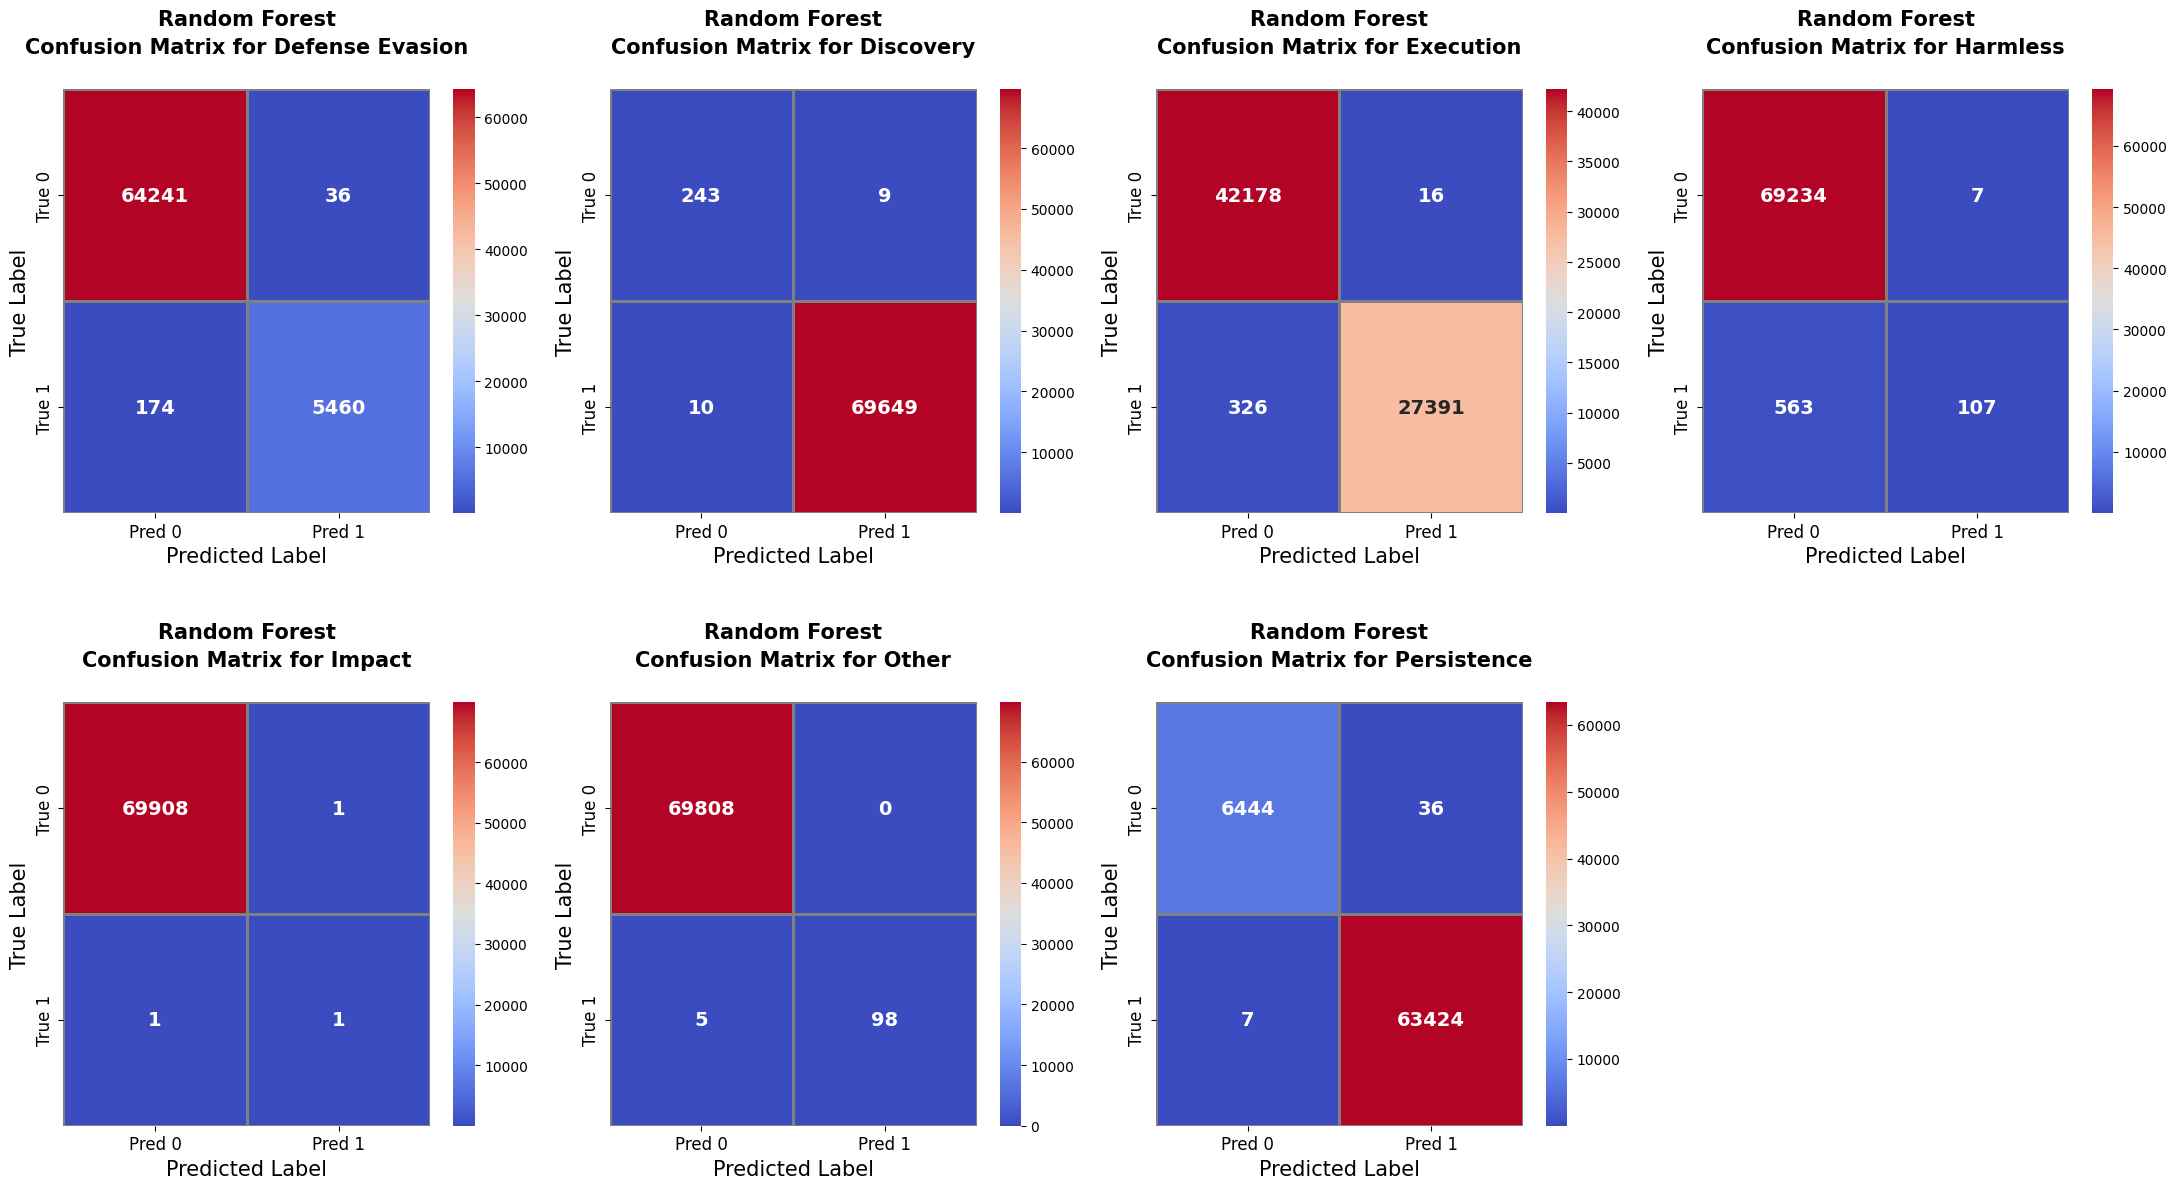
\includegraphics[width=0.77\textwidth]{../figures/plots/section2/Random_Forest_normalized_confusion_matrix_test.png}
                    \caption{Random Forest Confusion Matrices}
                    \label{fig:rf_cm_base}
                \end{minipage}%
            \end{minipage}

            \vspace{0.5cm}  % Add some vertical spacing between rows
            
            % Middle row  
            \begin{minipage}{\textwidth}
                % Middle-left (Train)
                \begin{minipage}[c]{0.48\textwidth}
                    \centering
                    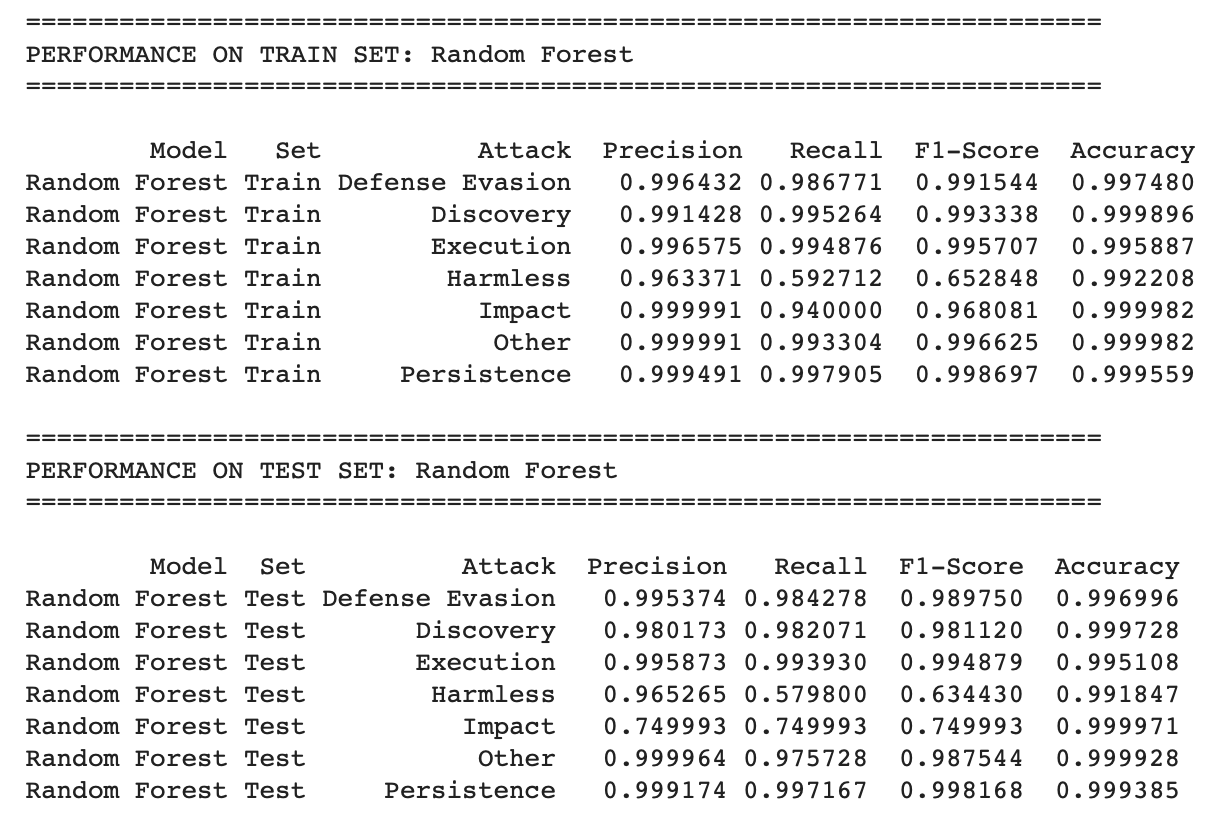
\includegraphics[width=0.9\textwidth]{../figures/plots/section2/Random_Forest_evaluation_metrics.png}
                    \caption{Random Forest Evaluation Metrics}
                    \label{fig:rf_em_base}
                \end{minipage}%
                \hfill%
                % Middle-right (Train)
                \begin{minipage}[c]{0.48\textwidth}
                    \centering
                    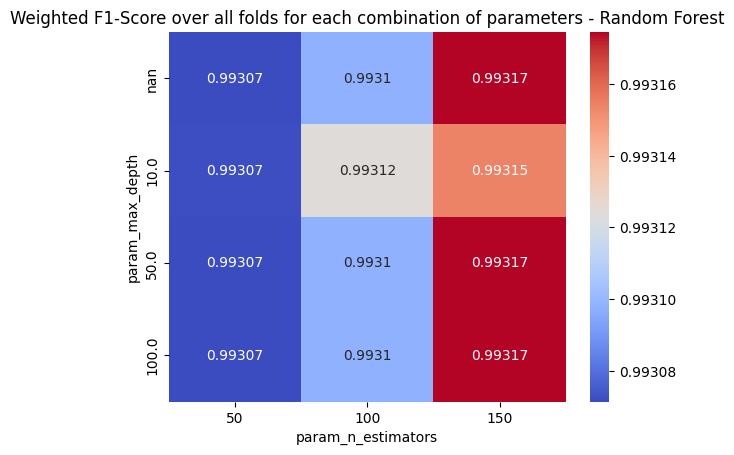
\includegraphics[width=0.7\textwidth]{../figures/plots/section2/weighted_f1_score_for_each_combination_of_parameters_random_forest.png}
                    \caption{Random Forest Weighted F1 Scores}
                    \label{fig:rf_f1_tuning}
                \end{minipage}
            \end{minipage}
            
            \vspace{0.5cm}  % Add some vertical spacing between rows

            % Bottom row
            \begin{minipage}{\textwidth}
                % Bottom-left (Test)
                \begin{minipage}[t]{0.48\textwidth}
                    \centering
                    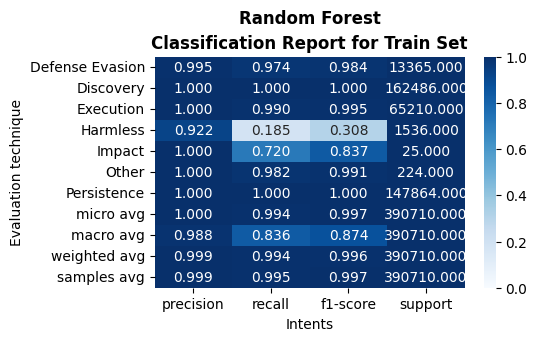
\includegraphics[width=0.9\textwidth]{../figures/plots/section2/Random_Forest_classification_report_for_Train_set.png}
                    \caption{Random Forest Classification Report Train Set}
                    \label{fig:rf_cm_train}
                \end{minipage}%
                \hfill%
                % Bottom-right (Test)
                \begin{minipage}[t]{0.48\textwidth}
                    \centering
                    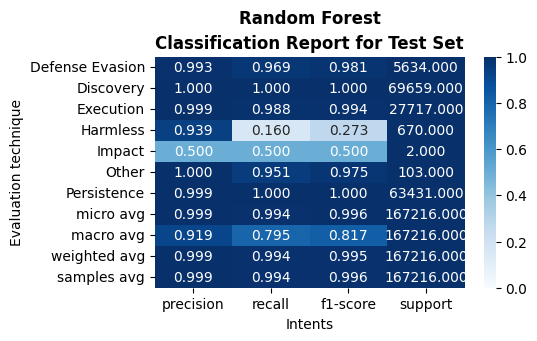
\includegraphics[width=0.9\textwidth]{../figures/plots/section2/Random_Forest_classification_report_for_Test_set.png}
                    \caption{Random Forest Classification Report Test Set}
                    \label{fig:rf_cm_test}
                \end{minipage}  
            
            \end{minipage}
            
        \end{figure}
            
        \clearpage
    
        % SVM
        
        \begin{figure}[H]
        
            \centering
            
            % Top row
            \begin{minipage}{\textwidth}
                \centering
                \begin{minipage}[c]{\textwidth}
                    \centering
                    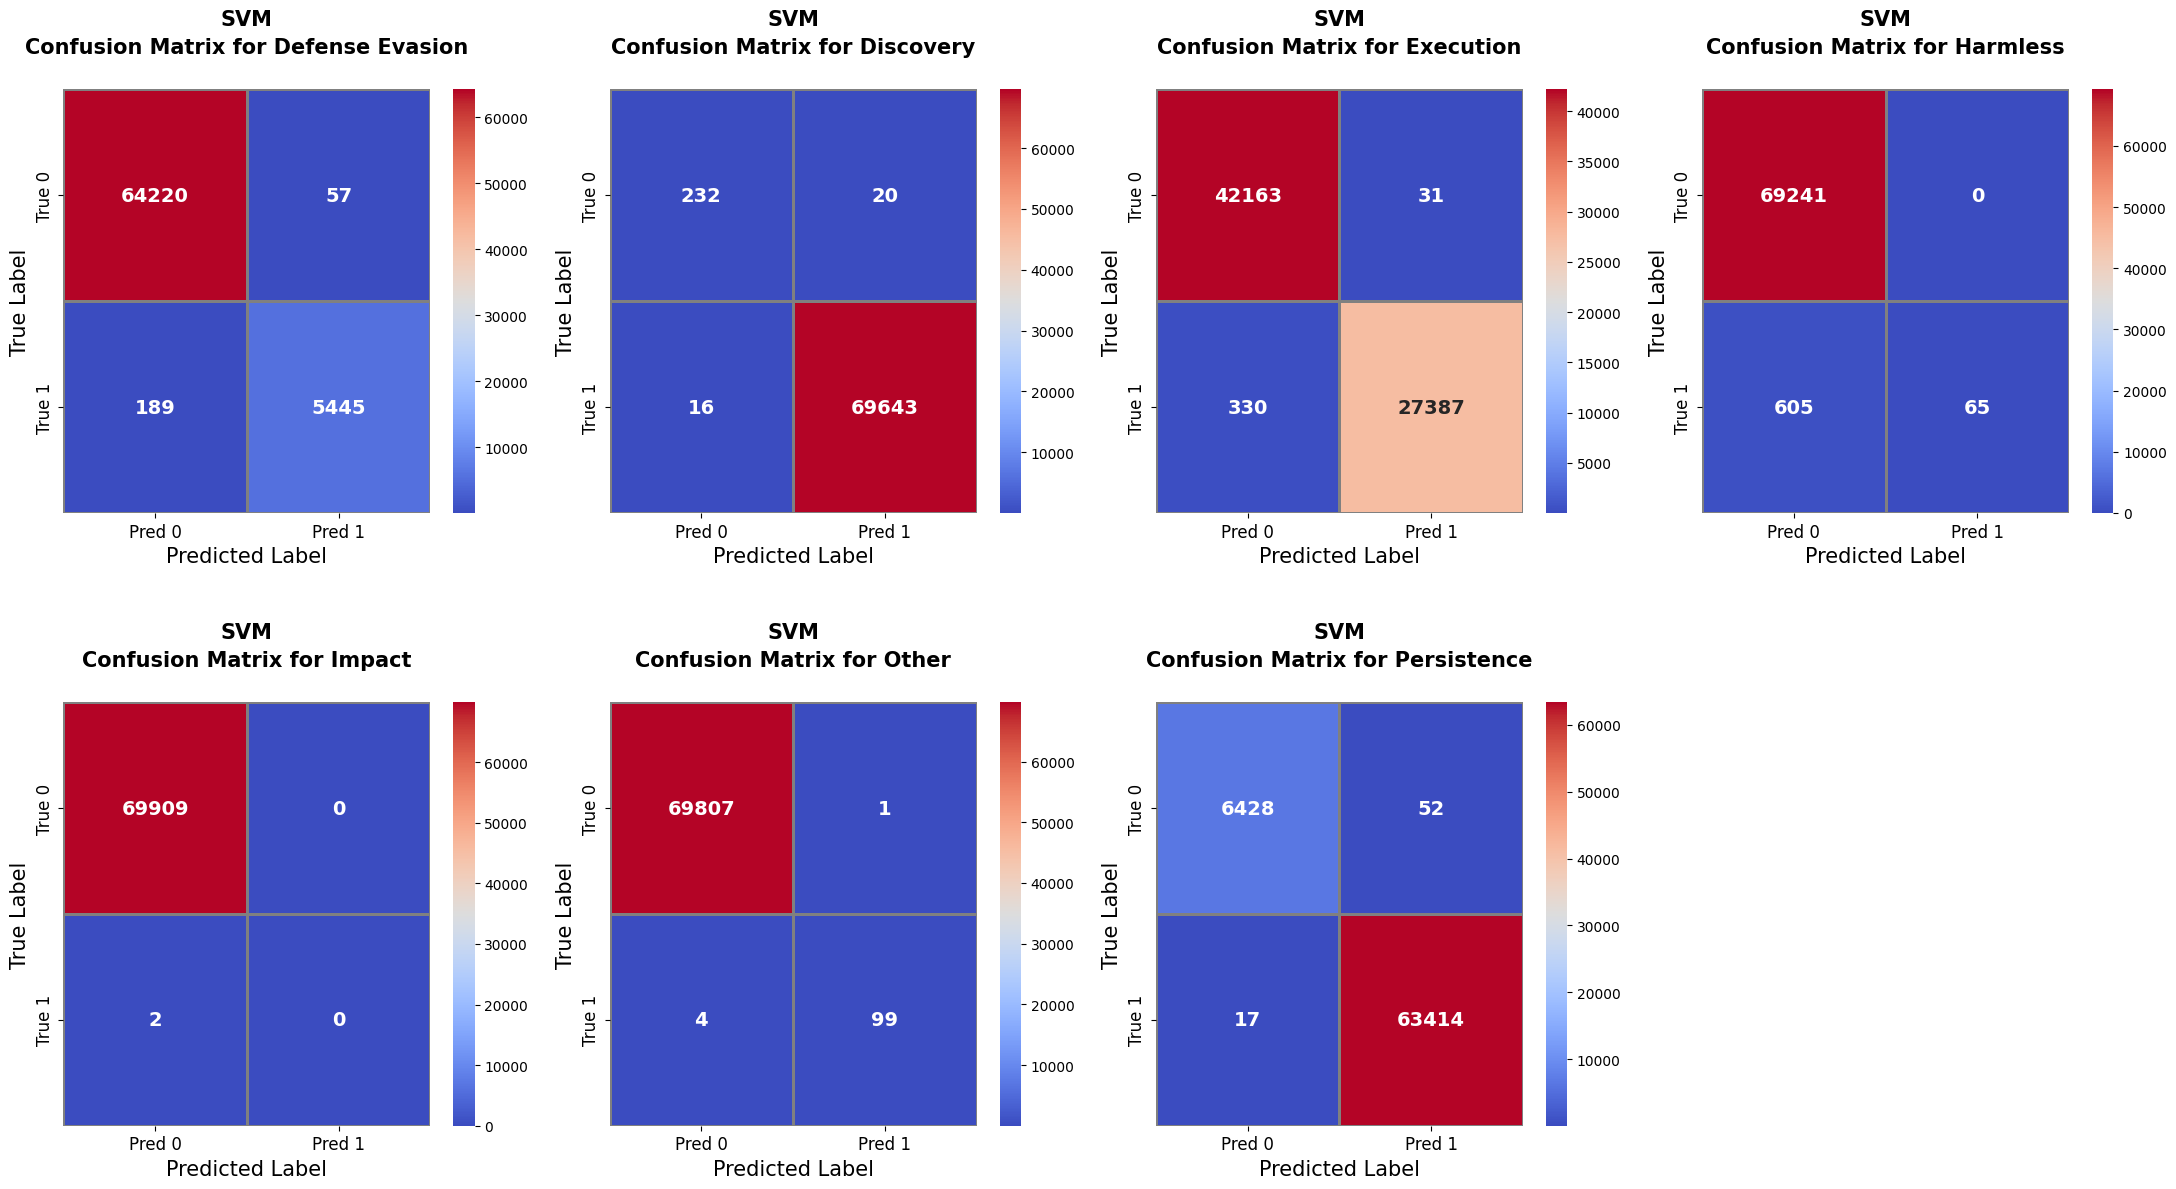
\includegraphics[width=0.77\textwidth]{../figures/plots/section2/SVM_normalized_confusion_matrix_test.png}
                    \caption{SVM Confusion Matrices}
                    \label{fig:svm_cm_base}
                \end{minipage}%
            \end{minipage}

            \vspace{0.5cm}  % Add some vertical spacing between rows
            
            % Middle row  
            \begin{minipage}{\textwidth}
                % Middle-left (Train)
                \begin{minipage}[c]{0.48\textwidth}
                    \centering
                    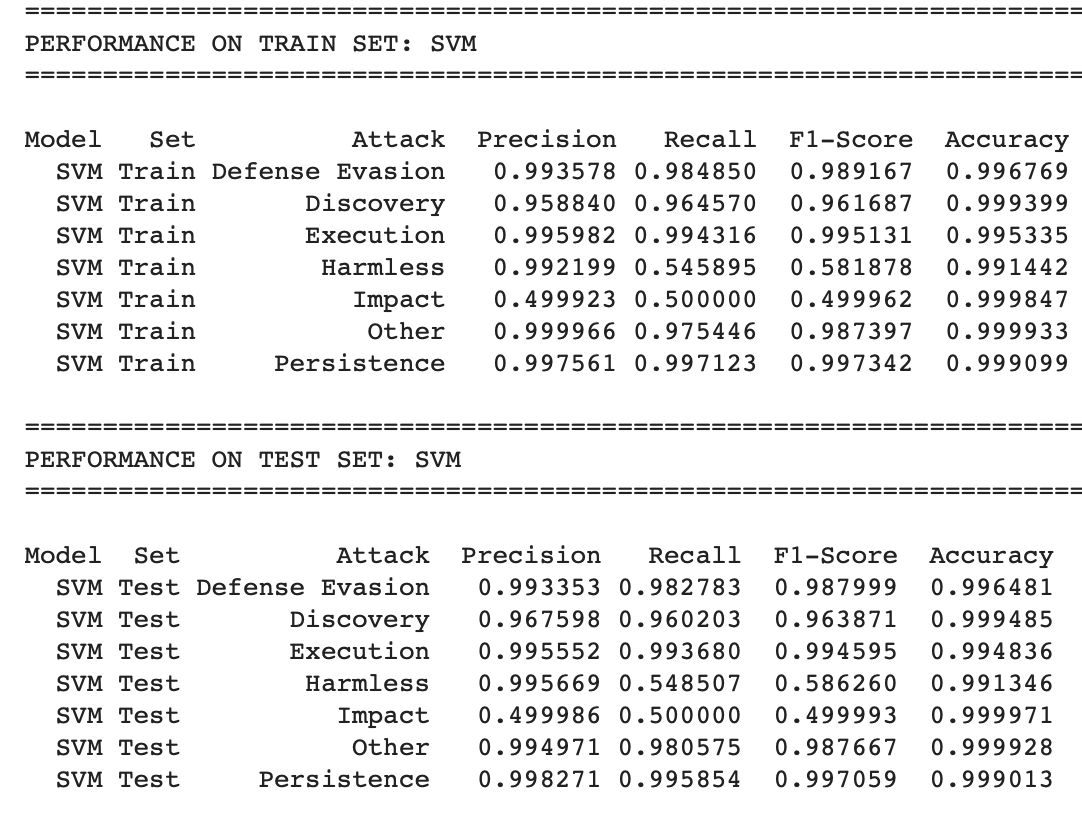
\includegraphics[width=0.8\textwidth]{../figures/plots/section2/SVM_evaluation_metrics.png}
                    \caption{SVM Evaluation Metrics}
                    \label{fig:svm_em_base}
                \end{minipage}%
                \hfill%
                % Middle-right (Train)
                \begin{minipage}[c]{0.48\textwidth}
                    \centering
                    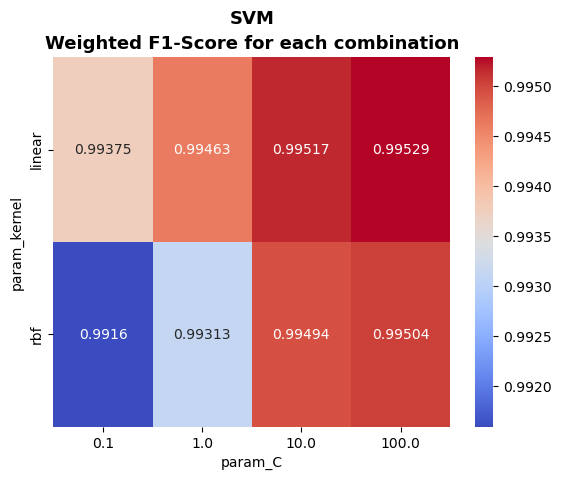
\includegraphics[width=0.7\textwidth]{../figures/plots/section2/weighted_f1_score_for_each_combination_of_parameters_svm.png}
                    \caption{SVM Weighted F1 Scores}
                    \label{fig:svm_f1_tuning}
                \end{minipage}
            \end{minipage}
            
            \vspace{0.5cm}  % Add some vertical spacing between rows

            % Bottom row
            \begin{minipage}{\textwidth}
                % Bottom-left (Test)
                \begin{minipage}[t]{0.48\textwidth}
                    \centering
                    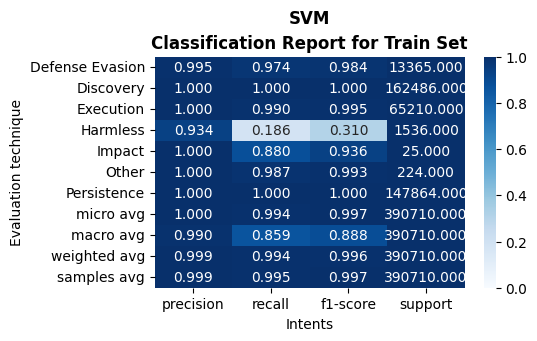
\includegraphics[width=0.9\textwidth]{../figures/plots/section2/SVM_classification_report_for_Train_set.png}
                    \caption{SVM Classification Report Train Set}
                    \label{fig:svm_cm_train}
                \end{minipage}%
                \hfill%
                % Bottom-right (Test)
                \begin{minipage}[t]{0.48\textwidth}
                    \centering
                    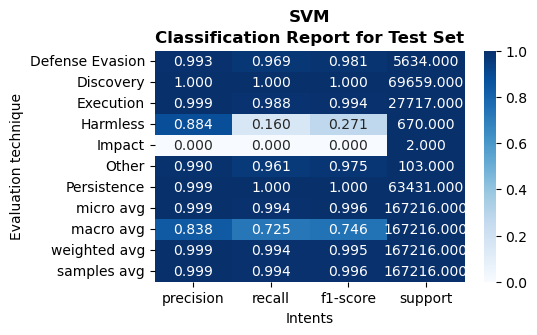
\includegraphics[width=0.9\textwidth]{../figures/plots/section2/SVM_classification_report_for_Test_set.png}
                    \caption{SVM Classification Report Test Set}
                    \label{fig:svm_cm_test}
                \end{minipage}  
            
            \end{minipage}
            
        \end{figure}
